\section{Implications for the study and optimization of \acs{WCA}}\label{sec:implications}
\todo[inline]{Implications for task durations, wrt to naive scheme.}
\todo[inline]{Implications for optimization in terms of sampling, energy.}
\todo[inline]{Introduction to this section}

\subsection{Application lifetimes}

We begin by studying the implications of such a model on the estimation of application lifetimes.
In the context of \ac{WCA}, we will understand \emph{application lifetime} as the time it takes a user to complete a specified task.
This is an important metric for \ac{WCA} optimization, as it directly relates to system resource utilization and contention, and to energy consumption.

In order to illustrate the consequences of using a less realistic model which does not take into account higher order effects, we introduce here a reference model to which we will compare our more realistic models.
This new model represents a first-order approximations the empirical execution time modeling, and consist simply of an \ac{exGaussian} distribution fitted to all execution time samples collected for \textcite{olguinmunoz:impact2021}.
This distribution is then randomly sampled at runtime to obtain execution times for each step, without any sort of adjustment to the current state of the system.

We start by studying application lifetimes in a controlled, ideal setup by using the timing models to generate execution times for sequences of \num{100} steps subject to constant \acp{TTF}.
These runs are completely simulated and no sampling of video frames is performed; for each step, we simply feed the models a predefined \acp{TTF} and record the generated execution time.
We use the combination of \acp{TTF} and execution times to calculate theoretical step duration times and subsequent total application lifetimes.
This is done for \num{25} linearly distributed \acp{TTF} in the \SIrange[]{0}{5}{\second} range; \num{45} independent repetitions for each combination of model configuration and \ac{TTF}.

\begin{figure}
    \centering
    \begin{subfigure}[]{\columnwidth}
        \centering
        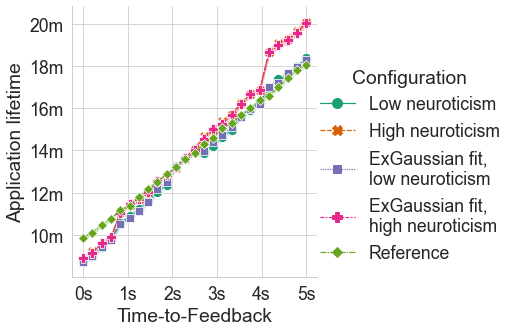
\includegraphics[width=.9\textwidth]{figs/new_model/lifetime_all_ttfs.png}
        \caption{%
            Evolution of application lifetimes as \acp{TTF} increase.
            Error bars indicate \SI{95}{\percent} \acp{CI}.
        }
    \end{subfigure}
    \begin{subfigure}[]{\columnwidth}
        \centering
        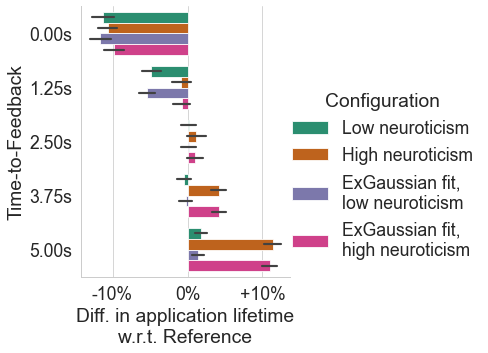
\includegraphics[width=.9\textwidth]{figs/new_model/lifetime_diff.png}
        \caption{%
            Percentage difference in mean application lifetimes with respect to the reference model at select \acp{TTF}.
            Error bars indicate the \SI{95}{\percent} \acp{CI}, calculated using a two-sided T-test.
        }
    \end{subfigure}
    \caption{\acl{TTF} versus application lifetime.}\label{fig:lifetimes}
\end{figure}

The results of this investigation are presented in \cref{fig:lifetimes}.
Compared to the reference model, our realistic models are, on average, roughly \SI{11}{\percent} faster when subject to low \acp{TTF}.
Conversely, at higher \acp{TTF} the relationship inverts, with the realistic models resulting in durations about \SI{2}{\minute} longer than the reference model, an increase of roughly \SI{11}{\percent}.

\todo[inline]{Discuss}

\begin{figure}
    \centering
    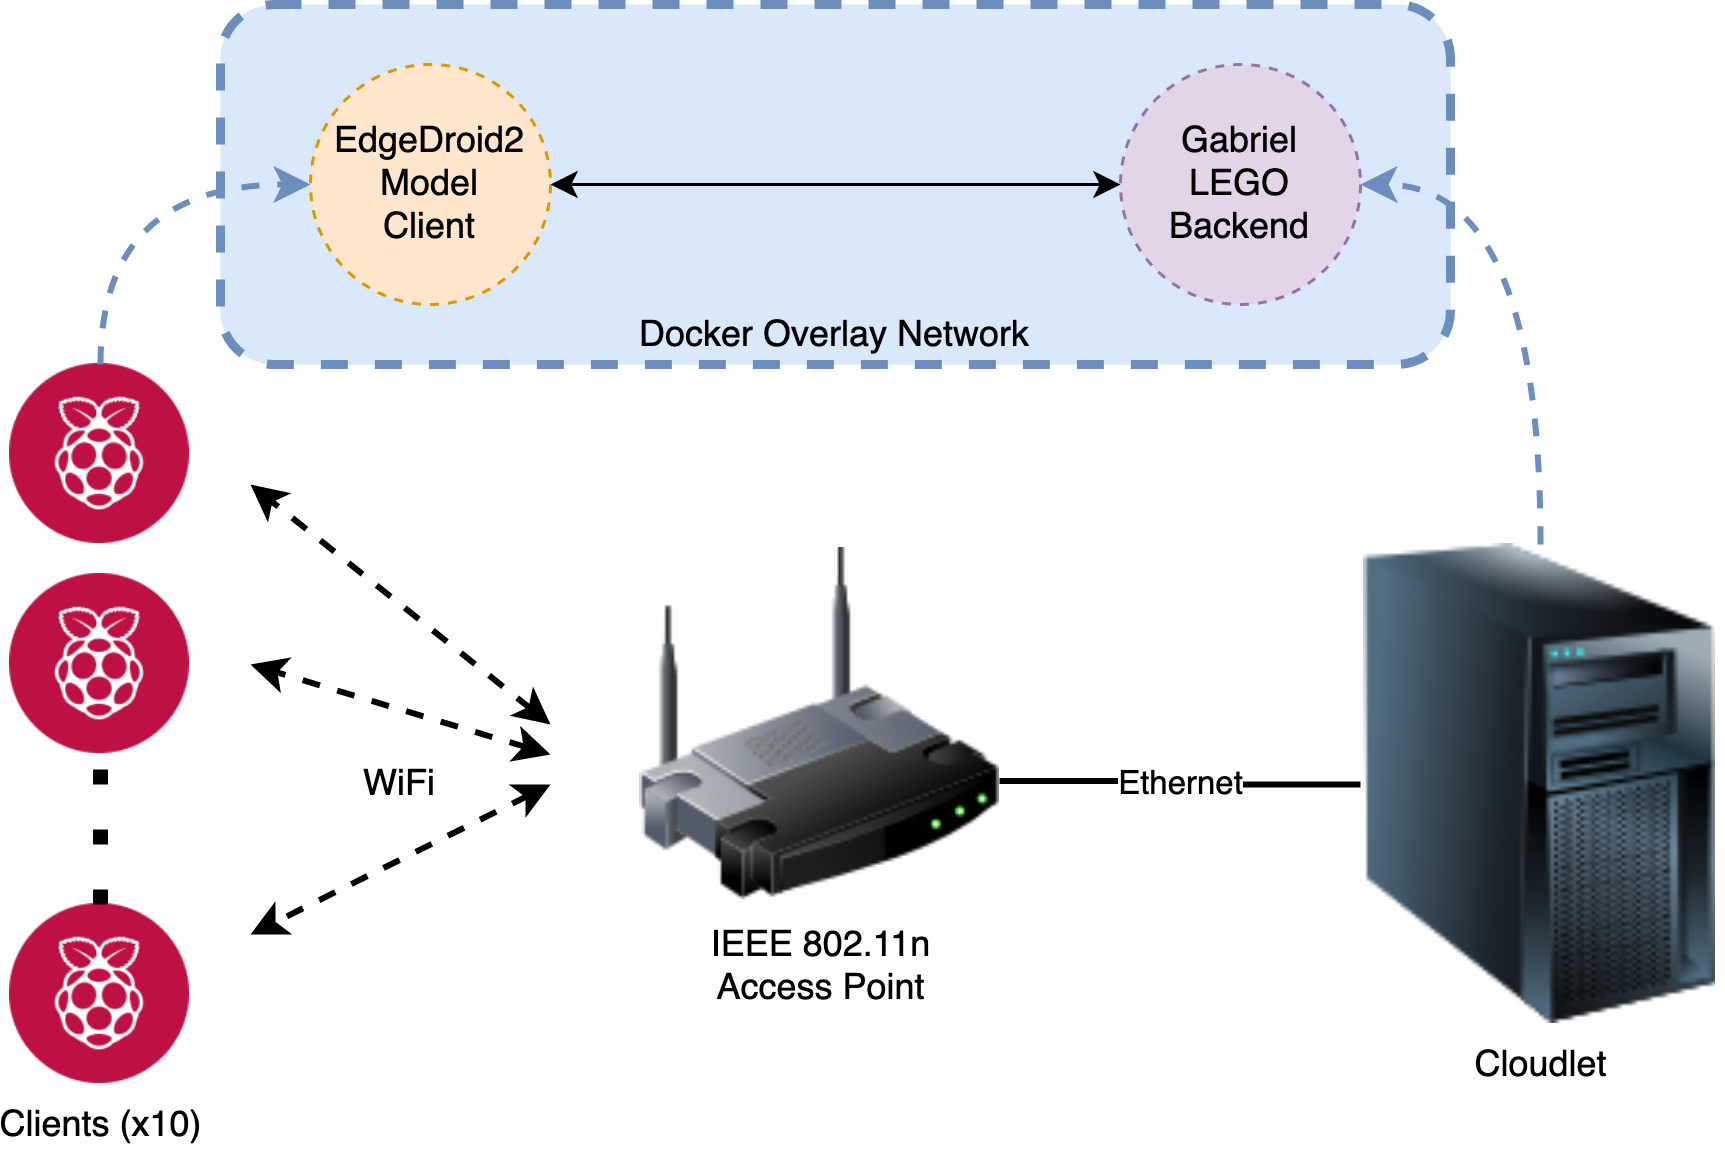
\includegraphics[width=\columnwidth]{figs/EdgeDroid2ExperimentalSetup.png}
    \caption{%
        Experimental setup used to study the implications of the realistic models of human behavior for \ac{WCA}.
        We deploy containerized instances of the client-server loop running the models on a testbed consisting of \num{10} Raspberry Pi clients connected to a cloudlet over a \ac{COTS} \acs{IEEE} \num{802.11}b/g access point.
    }\label{fig:expsetup}
\end{figure}

Next we study the effects of first- versus second-order models in a realistic setting.

\subsection{Optimizing for mean number of samples per step}

In~\cite{Wang2019Towards}, \citeauthor{Wang2019Towards} introduce an adaptive sampling scheme for \ac{WCA} intended to reduce the number of samples processed per step while still meeting application responsiveness bounds.
At every sampling instant \( t \), the scheme adapts the sampling rate \( R(t) \) of the system according to the estimated likelihood of the user having finished the step,
following the formula 

\begin{equation}
    R(t) = R_\text{min} + \alpha\left( R_\text{max} - R_\text{min} \right) * CDF(t)
\end{equation}

\( R_\text{max} \) and \( R_\text{min} \) correspond to the maximum and minimum sampling rates of the system, respectively.
\( R_\text{max} \) can directly be assumed to correspond to one over the mean \ac{RTT} of the system, whereas \( R_\text{min} \) needs to either be calculated according to the latency bounds of the system or specified manually.
\( \alpha \) corresponds to a scaling factor and \( t \) to the time of the current sampling instant with respect to the start of the step.
Finally, \( CDF \) corresponds to the \acl*{CDF} of a distribution describing the execution times for the current step; \citeauthor{Wang2019Towards} used a single static Gaussian distribution for all steps in their work.

In the following, we will show the effects of more accurate execution time estimation using our timing models on the performance of this adaptive scheme.
For this, we implement two variants of the adaptive scheme.
The first one corresponds to \citeauthor{Wang2019Towards}'s original design, using a Gaussian distribution fitted to all the execution times collected for~\cite{olguinmunoz:impact2021} for \ac{CDF} calculation.
The second variant instead uses an embedded internal execution time model to keep track of the \acp{TTF} of the system and adjust the distribution of execution times following the state of the timing model.

We proceed to set up an experiment where these sampling scheme variants are deployed on identical, simulated, \num{100}-step tasks.
The execution times for each step are generated by a realistic model parameterized with high neuroticism and without any distribution fitting on the data (this timing model is separate from the internal timing models inside the sampling schemes).
We set \( R_\text{min} \) to \SI{0.5}{\hertz}, \( \alpha \) to \num{3.0}, and the \ac{RTT} of the system to a constant \SI{150}{\milli\second}, and then run \num{90} repetitions of the task for the original design of the sampling scheme as well as for each possible configuration of it with a different parameterization of the timing model.

\begin{figure}
    \centering
    \begin{subfigure}[]{\columnwidth}
        \centering
        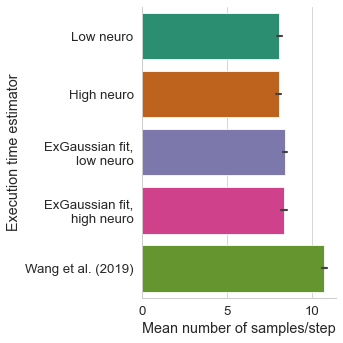
\includegraphics[width=.9\textwidth]{figs/new_model/sampling_junjue.png}
        \caption{%
            Mean number of samples per step over a \num{100}-step task, \num{90} independent repetitions per configuration.
            Error bars indicate \SI{95}{\percent} \acp{CI}.
        }
    \end{subfigure}
    \begin{subfigure}[]{\columnwidth}
        \centering
        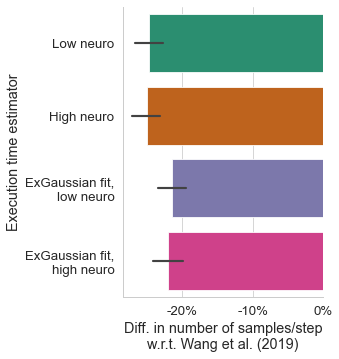
\includegraphics[width=.9\textwidth]{figs/new_model/diff_sampling_junjue.png}
        \caption{%
            Percentage difference in mean number of samples per step.
            Error bars indicate the \SI{95}{\percent} \acp{CI}, calculated using a two-sided T-test.
        }
    \end{subfigure}
    \caption{Results of parameterizing \textcite{Wang2019Towards}'s adaptive sampling scheme using the realistic timing model.}\label{fig:samples}
\end{figure}

The results of this investigation are presented in \cref{fig:samples}, and they clearly show the potentially dramatic effects of more accurate execution time estimation when optimizing sampling rates.
When using the realistic model for execution time estimation, the sampling scheme achieve between \SI{21}{\percent} and \SI{25}{\percent} better average performance.
This is true even for configurations with low neuroticism which do not exactly match the parameterization of the external timing model driving the execution times for the steps, showing thus the importance of even less-accurate approximations.

\subsection{Optimizing for energy consumption}

\todo[inline]{Add description of aperiodic sampling scheme}